\documentclass[11pt,letterpaper]{article}
\usepackage{acl-hlt2011}
\usepackage{thanks-nostar}
\usepackage{subfig}
%\setlength\titlebox{3in}
%\usepackage{naaclhlt2010}
%\usepackage{draftcopy}[all,draft,light,timestamp]
%\usepackage{draftwatermark}
\usepackage{datetime}
\usepackage{times}
\usepackage{latexsym}
\usepackage{url}
\usepackage{multirow}
\usepackage{amsmath}
\usepackage{bm}
\usepackage{todonotes}
\usepackage{algorithm}
\usepackage{algpseudocode}
\usepackage{tikz}
\usepackage{pgfplots}
\pgfplotsset{
width=7cm,
compat=1.3,
colormap name=blackwhite
%,bar cycle list name=black white
}
%\SetWatermarkLightness{0.95}
%\SetWatermarkLightness{1}
%\SetWatermarkText{\dmyydate \today, \currenttime}
\DeclareMathOperator*{\argmax}{arg\,max}



\title{How to Split Data to Speed Up MERT}

\author{Lane Schwartz\\
  Air Force Research Laboratory\\
  Human Effectiveness Directorate\\
  Wright-Patterson AFB, OH USA
}



\begin{document}
\maketitle

%%%%%%%%%%%%%%%%%%%%%%%
% Let's find some space
\renewcommand{\topfraction}{0.9}
\renewcommand{\bottomfraction}{0.8}
\renewcommand{\textfraction}{0.05}
\renewcommand{\dbltopfraction}{0.9}
\renewcommand{\dblfloatpagefraction}{0.9}
\setcounter{topnumber}{10}
\setcounter{bottomnumber}{10}
\setcounter{totalnumber}{10}
\setcounter{dbltopnumber}{10}
%
%%%%%%%%%%%%%%%%%%%%%%%



\begin{abstract}
Each iteration of minimum error rate training involves re-translating a development set. Distributing this work across computational nodes can speed up translation time, but in practice some parts may take much longer to complete than others, leading to computational slack time. To address this problem, we develop three novel algorithms for distributing translation tasks in a parallel computing environment, drawing on research in parallel machine scheduling. We present results showing a substantial speedup in overall decoding time.
\end{abstract}



\section{Introduction}

The task of translation involves translating a source language document $\mathbf{f}$ into target language $\mathbf{e}$. Most popular statistical translation techniques select the best translation $\hat{e}$ for source sentence $f$ according to a linear combination of models $\bm{\phi}$ using a set of model weights $\bm{\lambda}$ \cite{ochney02}. 

\begin{equation}
\hat{e} = \argmax_e \sum_i \lambda_i \phi_i(e,f)
\label{eq:smt}
\end{equation}


Values for $\bm{\lambda}$ are obtained by optimizing an objective function such as BLEU \cite{papinenietal01} against a development set, most commonly using minimum error rate training (MERT) \cite{och03}. Each iteration of MERT requires this development set to be re-translated using a new set of $\bm{\lambda}$ weights. MERT is one of the slowest components in a typical machine translation training pipeline, and translating the development set is nearly always the slowest step in MERT. We now examine techniques for speeding up MERT by distributing translation jobs across a cluster of parallel computational nodes. 

Ideally, all parts should take the same amount of time to translate. While naive splitting techniques reduce the time required for each translation iteration by splitting the work between $p$ computational nodes, in practice some parts may take much longer to complete than others. This can lead to significant computational slack time.
%
To address this problem, we develop three novel algorithms for splitting translation tasks in a parallel computing environment, drawing on research in parallel machine scheduling.





\section{Related Work}

While the models in Equation \ref{eq:smt} could, in theory, condition on previously translated sentences, in practice virtually no widely used models do so. It is therefore very straightforward to split the data into $p$ parts, and translate each part independently on $p$ computational nodes. Scripts implemented in Moses \cite{moses} do exactly that, simply splitting the data into $p$ arbitrary parts such that each part contains the same number of lines (Algorithm \ref{alg:naive}).

\begin{algorithm}
\caption{Split input text into $n$ parts such that each part contains the same number of lines.}
\begin{algorithmic}
\Function{Naive-Split}{$n$,input}
\State $\ell \gets n / $ input.length
\For {$p \gets 0 \ldots (n-1)$}
\State $i \gets \ell \times p$
\For {$j \gets i \ldots (i+\ell-1)$}
\If{$j < \ell$}
\State output[$p$].append(input[$j$])
\Else
\State \textbf{break}
\EndIf
\EndFor
\EndFor
\State \textbf{return} output
\EndFunction
\end{algorithmic}
\label{alg:naive}
\end{algorithm}


Research into parallel machine scheduling problems constitutes a wide and well-studied field, ranging through various disciplines of engineering, manufacturing, and management in addition to computer science and applied mathematics \cite{ChengSin90}, 
spanning a wide range of scheduling techniques \cite{PanwalkarIskander77}.
%\newcite{PanwalkarIskander77} present a survey of over 100 published scheduling techniques.

%In the general case, scheduling algorithms must determine where and when to schedule the execution of incoming jobs, based on machine factors such as the number of available machines, processing speed, memory availability, and the homogeneity or heterogeneity of available machines; and job factors such as arrival time, estimated work time, deadline, and whether or not jobs are preemptive. Preemptive jobs can be suspended during execution and later resumed on the a potentially different machine.

%Since we are interested in minimizing the overall runtime required to translate a source document (multiple times in the case of MERT), we are able to focus the range of above factors. The jobs in our task are treated as non-preemptive. Unlike the online variants of machine scheduling, all jobs in our task arrive simultaneously. These jobs have no explicit deadline. We further make the simplifying assumption that all execution hosts will be homogenous, with identical hardware configurations. 

We now briefly examine the existing research most relevant to our task. \newcite{Hu61} and Graham \shortcite{Graham66,Graham69} develop various list scheduling algorithms. This family of algorithms prioritizes jobs into a queue, then assigns jobs to machines in queue order. This approach attempts to evenly balance the load on each execution host \cite{DeMorton80,ChengSin90}. 
%Of the techniques which we examine in this work, Algorithms \ref{alg:naive}, \ref{alg:words}, and \ref{alg:times} fall into this category.
Both Algorithm \ref{alg:naive} and techniques we develop fall into this family of algorithms.


\begin{figure*}
\centering
\subfloat[Decoding times in \textbf{seconds} for standard decoder configured using a 5-gram language model.]{
%%%%%%%%%%%%%%%%%%%%%%% 
% Begin subfloat
%%%%%%%%%%%%%%%%%%%%%%%
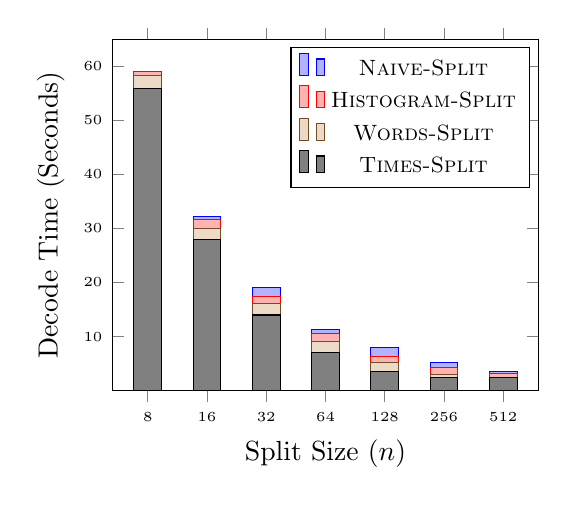
\begin{tikzpicture}
\begin{axis}[
xmode=log,
ymode=normal,
xtick=data,
ytick=data,
log basis x=2,
xticklabels={8,16,32,64,128,256,512},
ytick={160,150,140,130,120,110,100,90,80,70,60,50,40,30,20,10},
tick label style={font=\tiny},
xlabel=Split Size ($n$),
ylabel=Decode Time (Seconds),
ymin=0,
%legend style={
%	at={(0.5,-0.15)},
%	anchor=north,legend columns=-1
%},
ybar=0pt,
%bar width=3pt,
bar shift=0pt
]
%
\addplot
coordinates{
(8,58.41)
(16,32.24)
(32,19.14)
(64,11.28)
(128,7.98)
(256,5.27)
(512,3.61)
};

\addplot
coordinates{
(8,59.02)
(16,31.72)
(32,17.34)
(64,10.57)
(128,6.29)
(256,4.28)
(512,3.13)
};

\addplot
coordinates{
(8,58.28)
(16,29.96)
(32,16.07)
(64,9.05)
(128,5.16)
(256,2.95)
(512,2.5)
};

\addplot
coordinates{
(8,55.92)
(16,27.96)
(32,13.99)
(64,7.01)
(128,3.55)
(256,2.5)
(512,2.5)
};

%
\legend{{\footnotesize \sc Naive-Split},{\footnotesize \sc Histogram-Split},{\footnotesize \sc Words-Split},{\footnotesize \sc Times-Split}}
\end{axis}
\end{tikzpicture}
}
%%%%%%%%%%%%%%%%%%%%%%% 
% End subfloat
%%%%%%%%%%%%%%%%%%%%%%%
%
\qquad
%
%%%%%%%%%%%%%%%%%%%%%%% 
% Begin subfloat
%%%%%%%%%%%%%%%%%%%%%%%
\subfloat[Decoding times in \textbf{hours} for decoder configured using a syntactic language model (Schwartz et al., 2011) in addition to a 5-gram language model.]{
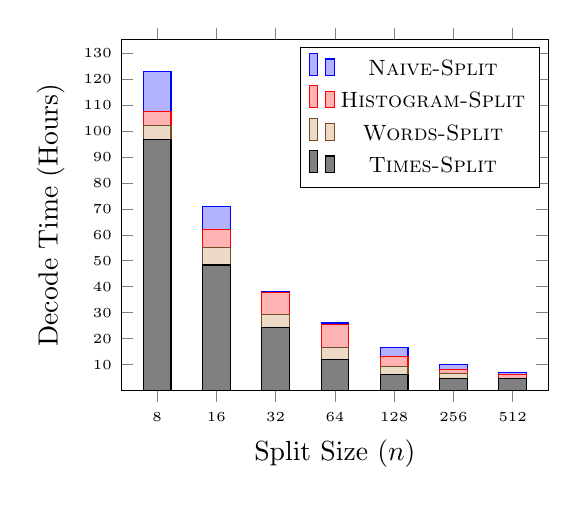
\begin{tikzpicture}%[scale=2]
\begin{axis}[
xmode=log,
ymode=normal,
xtick=data,
ytick=data,
log basis x=2,
xticklabels={8,16,32,64,128,256,512},
ytick={130,120,110,100,90,80,70,60,50,40,30,20,10},
tick label style={font=\tiny},
xlabel=Split Size ($n$),
ylabel=Decode Time (Hours),
ymin=0,
ybar=0pt,
bar shift=0pt
]
%
\addplot
coordinates{
(8,122.82107000000000000000)
(16,70.75433388888888888888)
(32,38.26489500000000000000)
(64,26.05343666666666666666)
(128,16.61346638888888888888)
(256,10.15095277777777777777)
(512,6.91079722222222222222)
};

\addplot
coordinates{
(8,107.64837166666666666666)
(16,61.96044666666666666666)
(32,37.76782722222222222222)
(64,25.39456444444444444444)
(128,13.00822500000000000000)
(256,8.02134666666666666666)
(512,6.30193611111111111111)
};

\addplot
coordinates{
(8,101.91934166666666666666)
(16,55.04415000000000000000)
(32,29.22364166666666666666)
(64,16.72757472222222222222)
(128,9.30142222222222222222)
(256,6.55191638888888888888)
(512,4.62488333333333333333)
};

\addplot
coordinates{
(8,96.72335333333333333333)
(16,48.36661722222222222222)
(32,24.20507777777777777777)
(64,12.12499472222222222222)
(128,6.17033611111111111111)
(256,4.62488333333333333333)
(512,4.62488333333333333333)
};

%
%\legend{Naive,Histogram,Words,Oracle}
\legend{{\footnotesize \sc Naive-Split},{\footnotesize \sc Histogram-Split},{\footnotesize \sc Words-Split},{\footnotesize \sc Times-Split}}
\end{axis}
\end{tikzpicture}
}
%%%%%%%%%%%%%%%%%%%%%%% 
% End subfloat
%%%%%%%%%%%%%%%%%%%%%%%
\caption{Decoding times for the slowest translation job in a translation task split into $n$ decoding jobs using various splitting algorithms ({\sc Naive-Split}, {\sc Histogram-Split}, {\sc Words-Split}, and {\sc Times-Split}).}
\label{fig:maxspeed}
\end{figure*}


\begin{figure*}
\centering
\subfloat[Decoding times in \textbf{seconds} for standard decoder configured using a 5-gram language model.]{
\begin{tabular} {| c || r | r || r | r || r | r || r | r |}
\hline
%\multirow{2}{*}{Split} 
Split Size & \multicolumn{2}{|c||}{\sc Naive-Split} & \multicolumn{2}{|c||}{\sc Histogram-Split} & \multicolumn{2}{|c||}{\sc Words-Split} & \multicolumn{2}{|c|}{\sc Times-Split} \\ \cline{2-9}
($n$) & \multicolumn{1}{|c|}{Min} & \multicolumn{1}{|c||}{Max} & \multicolumn{1}{|c|}{Min} & \multicolumn{1}{|c||}{Max} & \multicolumn{1}{|c|}{Min} & \multicolumn{1}{|c||}{Max} & \multicolumn{1}{|c|}{Min} & \multicolumn{1}{|c|}{Max} \\ \hline
2 & {222.9} & {224.4 } & {221.5} & {225.8 } & {219.3} & {228.0 } & \textit{223.7} & \textbf{\textit{223.7 }} \\ \hline
4 & {109.2} & {113.7 } & {110.0} & {114.6 } & {108.7} & {115.6 } & \textit{111.8} & \textbf{\textit{111.8 }} \\ \hline
8 & {51.4} & {58.4 } & {52.2} & {59.0 } & {53.2} & {58.3 } & \textit{55.9} & \textbf{\textit{55.9 }} \\ \hline
16 & {24.9} & {32.2 } & {25.0} & {31.7 } & {25.3} & {30.0 } & {27.9} & \textbf{28.0 } \\ \hline
32 & {11.3} & {19.1 } & {11.9} & {17.3 } & {11.7} & {16.1 } & \textit{14.0} & \textbf{\textit{14.0 }} \\ \hline
64 & {5.4} & {11.3 } & {5.4} & {10.6 } & {5.7} & {9.1 } & \textit{7.0} & \textbf{\textit{7.0 }} \\ \hline
128 & {1.3} & {8.0 } & {2.2} & {6.3 } & {2.3} & {5.2 } & \textit{3.5} & \textbf{\textit{3.5 }} \\ \hline
256 & {0.3} & {5.3 } & {0.7} & {4.3 } & {0.8} & {3.0 } & {1.7} & \textbf{2.5 } \\ \hline
512 & {0.0} & {3.6 } & {0.2} & {3.1 } & {0.3} & \textbf{2.5 } & {0.6} & \textbf{2.5 } \\ \hline
\end{tabular}

} \\
\subfloat[Decoding times in \textbf{hours} for decoder configured using a syntactic language model (Schwartz et al., 2011) addition to a 5-gram language model.]{
\begin{tabular} {| c || r | r || r | r || r | r || r | r |}
\hline
%\multirow{2}{*}{Split} 
 & \multicolumn{2}{|c||}{Algorithm 1} & \multicolumn{2}{|c||}{Algorithm 2} & \multicolumn{2}{|c||}{Algorithm 3} & \multicolumn{2}{|c|}{Algorithm 4} \\ 
Split Size & \multicolumn{2}{|c||}{\fontspec{TeX Gyre Pagella}\textsc{Naive-Split}} & \multicolumn{2}{|c||}{\fontspec{TeX Gyre Pagella}\textsc{Histogram-Split}} & \multicolumn{2}{|c||}{\fontspec{TeX Gyre Pagella}\textsc{Words-Split}} & \multicolumn{2}{|c|}{\fontspec{TeX Gyre Pagella}\textsc{Times-Split}} \\ \cline{2-9}
($n$) & \multicolumn{1}{|c|}{Min} & \multicolumn{1}{|c||}{Max} & \multicolumn{1}{|c|}{Min} & \multicolumn{1}{|c||}{Max} & \multicolumn{1}{|c|}{Min} & \multicolumn{1}{|c||}{Max} & \multicolumn{1}{|c|}{Min} & \multicolumn{1}{|c|}{Max} \\ \hline
2 & {365.7} & {408.0 } & {376.3} & {397.5 } & {386.1} & {387.6 } & \textit{386.9} & \fontspec{TeX Gyre Pagella}\textbf{\textit{386.9 }} \\ \hline
4 & {176.1} & {214.4 } & {186.8} & {205.0 } & {184.6} & {200.9 } & \textit{193.4} & \fontspec{TeX Gyre Pagella}\textbf{\textit{193.4 }} \\ \hline
8 & {84.6} & {122.8 } & {84.8} & {107.6 } & {88.4} & {101.9 } & \textit{96.7} & \fontspec{TeX Gyre Pagella}\textbf{\textit{96.7 }} \\ \hline
16 & {40.8} & {70.8 } & {40.5} & {62.0 } & {45.3} & {55.0 } & \textit{48.4} & \fontspec{TeX Gyre Pagella}\textbf{\textit{48.4 }} \\ \hline
32 & {19.2} & {38.3 } & {18.8} & {37.8 } & {20.5} & {29.2 } & \textit{24.2} & \fontspec{TeX Gyre Pagella}\textbf{\textit{24.2 }} \\ \hline
64 & {9.2} & {26.1 } & {9.2} & {25.4 } & {9.4} & {16.7 } & \textit{12.1} & \fontspec{TeX Gyre Pagella}\textbf{\textit{12.1 }} \\ \hline
128 & {2.7} & {16.6 } & {4.1} & {13.0 } & {3.7} & {9.3 } & {5.9} & \fontspec{TeX Gyre Pagella}\textbf{6.2 } \\ \hline
256 & {0.7} & {10.2 } & {1.3} & {8.0 } & {1.4} & {6.6 } & {2.9} & \fontspec{TeX Gyre Pagella}\textbf{4.6 } \\ \hline
512 & {0.0} & {6.9 } & {0.3} & {6.3 } & {0.6} & \fontspec{TeX Gyre Pagella}\textbf{4.6 } & {1.1} & \fontspec{TeX Gyre Pagella}\textbf{4.6 } \\ \hline
\end{tabular}

}
\caption{Decoding times for the fastest (min) and slowest (max) decoding jobs when a translation task is split into $n$ decoding jobs. \textit{Italics} indicate balanced task times. \textbf{Bold} indicates fastest max time at that split.}
\label{fig:minmaxspeed}
\end{figure*}




\begin{figure*}[!tb]
%%%%%%%%%%%%%%%%%%%%%%% 
% Begin subfloat
%%%%%%%%%%%%%%%%%%%%%%%
\subfloat[Slack \textbf{CPU-Seconds} for standard decoder configured using a 5-gram language model.]{
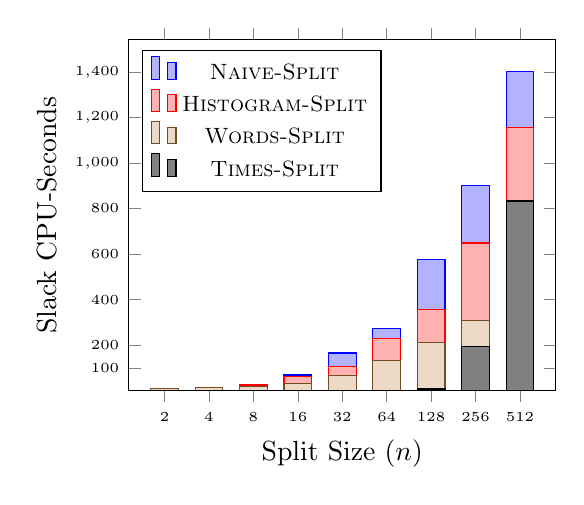
\begin{tikzpicture}
\begin{axis}[
xmode=log,
ymode=normal,
xtick=data,
ytick=data,
log basis x=2,
xticklabels={2,4,8,16,32,64,128,256,512},
scaled y ticks=false,
ytick={2000,1800,1600,1400,1200,1000,800,600,400,200,100},
tick label style={font=\tiny},
xlabel=Split Size ($n$),
ylabel=Slack CPU-Seconds,
ymin=0,
legend pos=north west,
ybar=0pt,
%bar width=3pt,
bar shift=0pt
]
%
\addplot
coordinates{
(2,1.55000000000001)
(4,7.37000000000002)
(8,19.97)
(16,68.53)
(32,165.17)
(64,274.61)
(128,574.13)
(256,901.81)
(512,1401.01)
};

\addplot
coordinates{
(2,4.26999999999998)
(4,11.01)
(8,24.85)
(16,60.21)
(32,107.57)
(64,229.17)
(128,357.81)
(256,648.37)
(512,1155.25)
};

\addplot
coordinates{
(2,8.64999999999998)
(4,15.05)
(8,18.93)
(16,32.05)
(32,66.93)
(64,131.89)
(128,213.17)
(256,307.89)
(512,832.689999999999)
};

\addplot
coordinates{
(2,0.00999999999999091)
(4,0.0100000000000051)
(8,0.0500000000000256)
(16,0.0500000000000078)
(32,0.369999999999992)
(64,1.32999999999998)
(128,7.08999999999998)
(256,192.69)
(512,832.690000000001)
};

%
\legend{{\footnotesize \sc Naive-Split},{\footnotesize \sc Histogram-Split},{\footnotesize \sc Words-Split},{\footnotesize \sc Times-Split}}
\end{axis}
\end{tikzpicture}
}
%%%%%%%%%%%%%%%%%%%%%%% 
% End subfloat
%%%%%%%%%%%%%%%%%%%%%%%
%
\qquad
%
%%%%%%%%%%%%%%%%%%%%%%% 
% Begin subfloat
%%%%%%%%%%%%%%%%%%%%%%%
\subfloat[Slack \textbf{CPU-Hours} for decoder configured using a syntactic language model (Schwartz et al., 2011) in addition to a 5-gram language model.]{
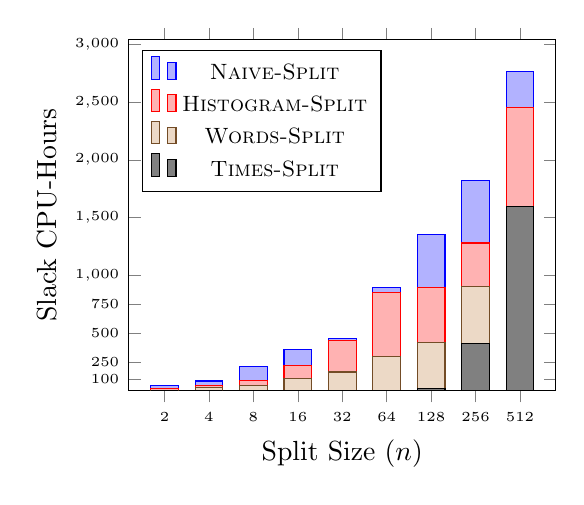
\begin{tikzpicture}
\begin{axis}[
xmode=log,
ymode=normal,
xtick=data,
ytick=data,
log basis x=2,
xticklabels={2,4,8,16,32,64,128,256,512},
ytick={3000,2500,2000,1500,1000,750,500,250,100},
tick label style={font=\tiny},
xlabel=Split Size ($n$),
ylabel=Slack CPU-Hours,
ymin=0,
legend pos=north west,
ybar=0pt,
%bar width=3pt,
bar shift=0pt
]
%
\addplot
coordinates{
(2,42.29704944444444444444)
(4,83.69433333333333333333)
(8,208.78464888888888888888)
(16,358.28543111111111111111)
(32,450.69272888888888888888)
(64,893.63603555555555555555)
(128,1352.73978666666666666666)
(256,1824.86000000000000000000)
(512,2764.54426666666944444444)
};

\addplot
coordinates{
(2,21.15789388888891666666)
(4,46.23076777777777777777)
(8,87.40306222222222222222)
(16,217.58323555555555555555)
(32,434.78656000000000000000)
(64,851.46821333333333333333)
(128,891.26888888888888888888)
(256,1279.68083555555555555555)
(512,2452.80737777777777777777)
};

\addplot
coordinates{
(2,1.49376777777778055555)
(4,29.94747777777777777777)
(8,41.57082222222222222222)
(16,106.92248888888888888888)
(32,161.37262222222222222222)
(64,296.78087111111111111111)
(128,416.79813333333333333333)
(256,903.50668444444444444444)
(512,1594.15635555555277777777)
};

\addplot
coordinates{
(2,.00000666666672461563)
(4,.00046666666661621944)
(8,.00291555555553511111)
(16,.08196444444438388888)
(32,.77857777777776666666)
(64,2.21575111111110277777)
(128,16.01911111111108333333)
(256,410.18622222222222222222)
(512,1594.15635555555555555555)
};

%
\legend{{\footnotesize \sc Naive-Split},{\footnotesize \sc Histogram-Split},{\footnotesize \sc Words-Split},{\footnotesize \sc Times-Split}}
\end{axis}
\end{tikzpicture}
}
%%%%%%%%%%%%%%%%%%%%%%% 
% End subfloat
%%%%%%%%%%%%%%%%%%%%%%%
\caption{Cumulative slack CPU time for $n$ processing cores when processing a parallel translation task split into $n$ jobs using various splitting algorithms. Slack CPU time is caused when some jobs finish before others. Zero slack time indicates conditions where all jobs complete simultaneously.}
\label{fig:slack}
\end{figure*}

\section{Better Splitting for Faster Results}

To observe the effects of splitting algorithms on decoding speed, we translated Urdu-English data using Moses in a parallel computing cluster, distributing work using the Sun Grid Engine. We ran two decoding setups: a standard configuration using a 5-gram language model, and a much slower syntactic LM configuration following \newcite{schwartzetal11}. Using Algorithm \ref{alg:naive}, the runtimes of the slowest of $n$ translation jobs in each configuration is illustrated in Figure \ref{fig:maxspeed} for various values of $n$. Figure \ref{fig:minmaxspeed} shows that in all cases, there is a significant difference between the fastest and slowest translation job, leading to computational slack time (Figure \ref{fig:slack}).

%While the models in Equation \ref{eq:smt} could, in theory, condition on previously translated sentences, in practice virtually no widely used models do so. It is therefore very straightforward to split the data into $p$ parts, and translate each part independently on $p$ computational nodes. The question then arises - how should the data be split? Algorithm \ref{alg:naive} naively splits the data into $p$ arbitrary parts such that each part contains the same number of lines. This algorithm is currently implemented and distributed in Moses \cite{moses}.

In examining these results, we observe that the slack time results primarily from situations where some jobs are assigned a disproportionate number of short sentences, and thus finish much faster than jobs that are assigned many longer sentences. To remedy this imbalance, we propose Algorithm \ref{alg:histogram}. This technique examines the word lengths of each sentence prior to splitting the data into jobs. Sentences are sorted according to length, then assigned in turns to jobs. This results in the sentence length histograms for each job being approximately equal. 
%
\begin{algorithm}[!t]
\caption{Split input text into $n$ parts to balance the histograms of line lengths for all parts.}
\begin{algorithmic}
\Function{Histogram-Split}{$n$,input}
\For {$i \gets 0 \ldots ($ input.length $-1)$}
\State sentence[$i$].length $\gets$ input[$i$].length
\State sentence[$i$].index $\gets i$
\EndFor
\State \Call{Sort}{sentence} $\left\{|x,y|\ x.\mbox{length}\Leftrightarrow y.\mbox{length}\right\}$ 
\State \Comment{Sort sentences by length}
\State $p \gets n$
\For {$i \gets 0 \ldots ($input.length $-1)$}
\If {$p < n$}
\State $p \gets p+1$
\Else
\State $p \gets 0$
\EndIf
\State output[$p$].append(input[sentence[$i$].index])
\EndFor
\State \textbf{return} output
\EndFunction
\end{algorithmic}
\label{alg:histogram}
\end{algorithm}
%
%
%In nearly all translation models, each sentence is translated independently 
%
%\todo[inline]{Describe Algorithm \ref{alg:words}. \\ \ \\ \ \\ \ \\ \ \\ \ \\ \ }
%
\begin{algorithm}[!t]
\caption{Split input text into $n$ parts to balance the number of words for all parts.}
\begin{algorithmic}
\Function{Words-Split}{$n$,input}
\For {$i \gets 0 \ldots ($ input.length $-1)$}
\State sentence[$i$].length $\gets$ input[$i$].length
\State sentence[$i$].index $\gets i$
\EndFor
\State \Call{Sort}{sentence} $\left\{|x,y|\ y.\mbox{length}\Leftrightarrow x.\mbox{length}\right\}$ 
\State \Comment{Sort sentences by length, in reverse order}
\For {$i \gets 0 \ldots ($ input.length $-1)$}
\State $p \gets$ \Call{Least}{words}
\State \Comment{Find partition with fewest words}
\State output[$p$].append(input[sentence[$i$].index])
\State words[$p$] $\gets$\hspace{0em}words[$p$] $+$ sentence[$i$].length%
%\State words[$p$]\hspace{0em}$\gets$\hspace{0em}words[$p$]\hspace{0em}$+$\hspace{0em}sentence[$i$].length%
\EndFor
\State \textbf{return} output
\EndFunction
\end{algorithmic}
\label{alg:words}
\end{algorithm}
%
Figures \ref{fig:maxspeed}a--\ref{fig:slack}a fail to show improvment in speed for a standard Moses configuration for small values of $n$. But for values of $n>8$, and for all values of $n$ using the slow syntactic language model (Figures \ref{fig:maxspeed}b--\ref{fig:slack}b), Algorithm \ref{alg:histogram} results in significant decreases in total decoding time over the naive Algorithm \ref{alg:naive}.

While Algorithm \ref{alg:histogram} balances short and long sentences across jobs, we may be able to improve runtimes by 
balancing the total number of words in each job. 
%
\begin{algorithm}[!t]
\caption{Split input text into $n$ parts to balance the estimated translation time of all parts.}
\begin{algorithmic}
\Function{Times-Split}{$n$,input,estimate}
\For {$i \gets 0 \ldots ($ input.length $-1)$}
\State sentence[$i$].time $\gets$ estimate[$i$]
\State sentence[$i$].index $\gets i$
\EndFor
\State \Call{Sort}{sentence} $\left\{|x,y|\ y.\mbox{time}\Leftrightarrow x.\mbox{time}\right\}$ 
\State \Comment{Sort sentences by time, in reverse order}
\For {$i \gets 0 \ldots ($ input.length $-1)$}
\State $p \gets$ \Call{Least}{times}
\State \Comment{Find partition with least time}
\State output[$p$].append(input[sentence[$i$].index])
\State times[$p$] $\gets$ times[$p$] $ + $ sentence[$i$].time
\EndFor
\State \textbf{return} output
\EndFunction
\end{algorithmic}
\label{alg:times}
\end{algorithm}
%
%
In Algorithm \ref{alg:words}, sentences are sorted by length into a queue, with longest sentences at the head of the queue.
%Algorithm \ref{alg:words} counts the number of words in each sentence to be translated. Sentences are then ordered by this length, in reverse order. Initially, no computation slots have assigned translation jobs. 
%
Initially, no sentences have been assigned to any job.
%
The longest sentence, at the head of the queue, is assigned first to a job. As each sentence is assigned to a job, the total number of words assigned to that job is recorded. 
%
Each subsequent sentence is removed from the queue and assigned to the job with 
%
%
the least work assigned to it, as measured by number 
%
of words.
%
Results for Algorithm \ref{alg:words} show substantial speedups over Algorithms \ref{alg:naive} and \ref{alg:histogram} when using the slower decoder configuration. Similar speedups are seen where $n>8$ for the faster configuration.



When assigning sentences to jobs, we would ideally like to know how long each sentence will take to process. Algorithms \ref{alg:histogram} and \ref{alg:words} use the number of words in each sentence as a proxy for processing time. During MERT, the same set of development sentences are translated multiple times. Since each decoding process differs only by the $\bm{\lambda}$ weights used, it is reasonable to expect similar runtimes for each run. With this in mind, we record the time required to translate each sentence during the first iteration of MERT. In subsequent iterations, Algorithm \ref{alg:times} uses the time recorded to translate a sentence as an estimate of the time it will take to translate that sentence again. Algorithm \ref{alg:times} differs from Algorithm \ref{alg:words} by sorting using these times instead of sentence length.
%\todo[inline]{Describe Algorithm \ref{alg:times}. \\ \ \\ \ \\ \ \\ \ \\ \ \\ \ \\ \ \\ \ \\ \ }
%
This technique results in speedups under all conditions (Figure \ref{fig:minmaxspeed}). In nearly all conditions, the speedup is substantial over the baseline. 
%
Slack time is at or near zero in all cases where $n<256$.
%Slack time is essentially eliminated in nearly all ($n<256$) conditions. 
%
%\footnote{Where slack time remains, $nabcheat=(256,512)$, a few jobs were each assigned a single long sentence that took longer to translate than the other jobs which were assigned multiple shorter sentences.}

%\vspace{-0.2cm}
\section{Conclusion}
\vspace{-0.1cm}

We have incorporated Algorithms \ref{alg:words} and \ref{alg:times} into 
the Moses decoding scripts,
%{\tt moses-parallel.pl},
% 
enabling substantial speed-ups in parallel decoding time at no additional cost.
%The use of Algorithm \ref{alg:words} in the first MERT iteration, and \ref{alg:times} in subsequent iterations.







% \begin{algorithm}
% \caption{Find the index of the smallest array element}
% \begin{algorithmic}
% \Function{Least}{array}
% \State best.value $\gets \infty$
% \State best.index $\gets 0$
% \For $i \gets 0 \ldots \mbox{array.length}-1$
% \If {array[$i$] $<$ best.value}
% \State best.value = array[$i$]
% \State best.index = $i$
% \EndIf
% \EndFor
% \State \textbf{return} best.index
% \EndFunction
% \end{algorithmic}
% \end{algorithm}




%\section{Conclusion}






%\todo[inline]{Describe results. \\ \ \\ \ \\ \ \\ \ \\ \ \\ \ \\ \ \\ \ \\ \ \\ \ \\ \ \\ \ }






\clearpage
\thanksnostar{Opinions, interpretations, conclusions, and recommendations are those of the authors and are not necessarily endorsed by the United States Air Force. Cleared for public release on 19 Jan 2011. Originator reference number RH-11-107802. Case number 88ABW-2011-0185.}
\bibliographystyle{acl}
\bibliography{bibliography}

\end{document}
